\section{Data synthesis}
\label{Datasynth}
To test our system, we simulated the movement of the IMU-camera system. We used noise-augmented versions of synthesized camera projections and IMU readings as input to the unscented Kalman filter. [[Andrew's synthesis goes here]].

We noticed that the above method produces a camera path where the camera does not consistently look at the points. The camera image plane might become parallel to the landmarks in world space, in which case, the points projections would lie at infinity. The camera may unrealistically look away from the points, or it may go too far from them. We needed a method that would produce a reasonable camera path, where the camera is within reach of the landmarks, and is consistently looking at them. In our second synthesis method, we manually defined control points of a Bezier curve around the $3D$ points, and we generated a smooth camera path using the Bezier curve. This path defined the position of the camera, $\bb{p}_C^W(t)$ at different instants of time. To specify the orientation $\hat{\overline{q}}_C^W(t)$, we computed a look at vector $v_{lookat}$ from the camera position $\bb{p}_C^W$ to the mean of the landmarks, $\bb{p}_{\mu}^C$. We defined an up vector, $v_{up}$ to lie along the $z$-axis by default, and we computed a third orthogonal vector, $v_{orth}=v_{lookat} \times v_{up}$. We computed the orientation in matrix form as $\begin{bmatrix}v_{orth} &v_{up}& v_{lookat}\end{bmatrix}$, and we converted it to the quaternion $\hat{\overline{q}}_C^W(t)$. Figure \ref{synthcontrolpts} shows the control points specified for the camera path, and Figure \ref{synthpath} shows the camera path as it looks at the points, the IMU attached rigidly to the camera, and the projected points in the camera's image plane.
\begin{figure}[t]
\centering
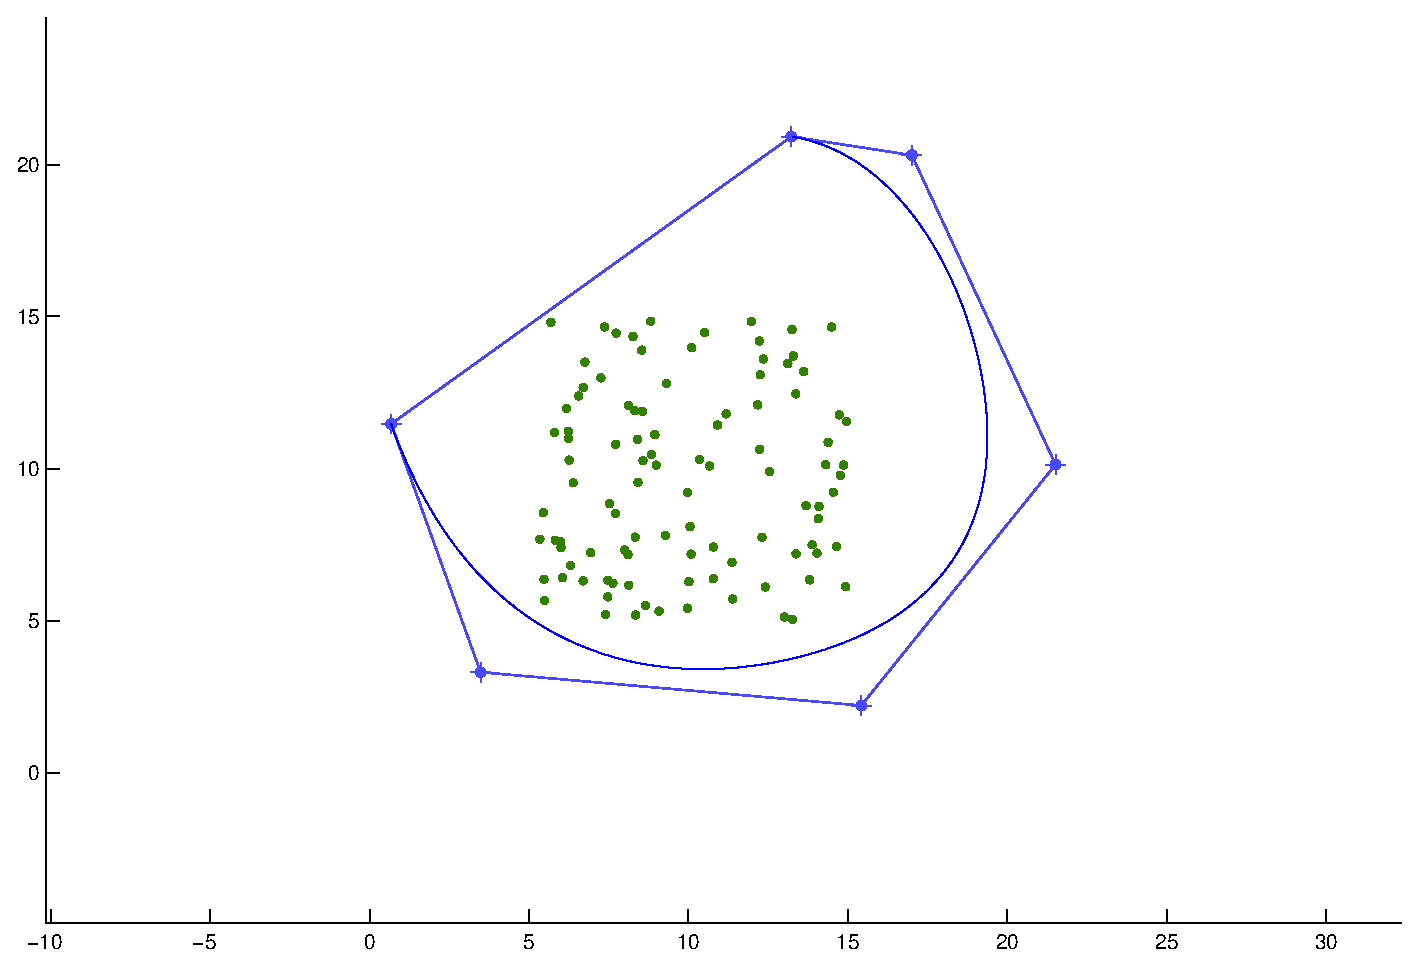
\includegraphics[width=.5\linewidth]{synth_controlpts.eps}
\caption{Top view of landmarks and control points used to generate camera path}
\label{synthcontrolpts}
\end{figure}
\begin{figure}[t]
\centering
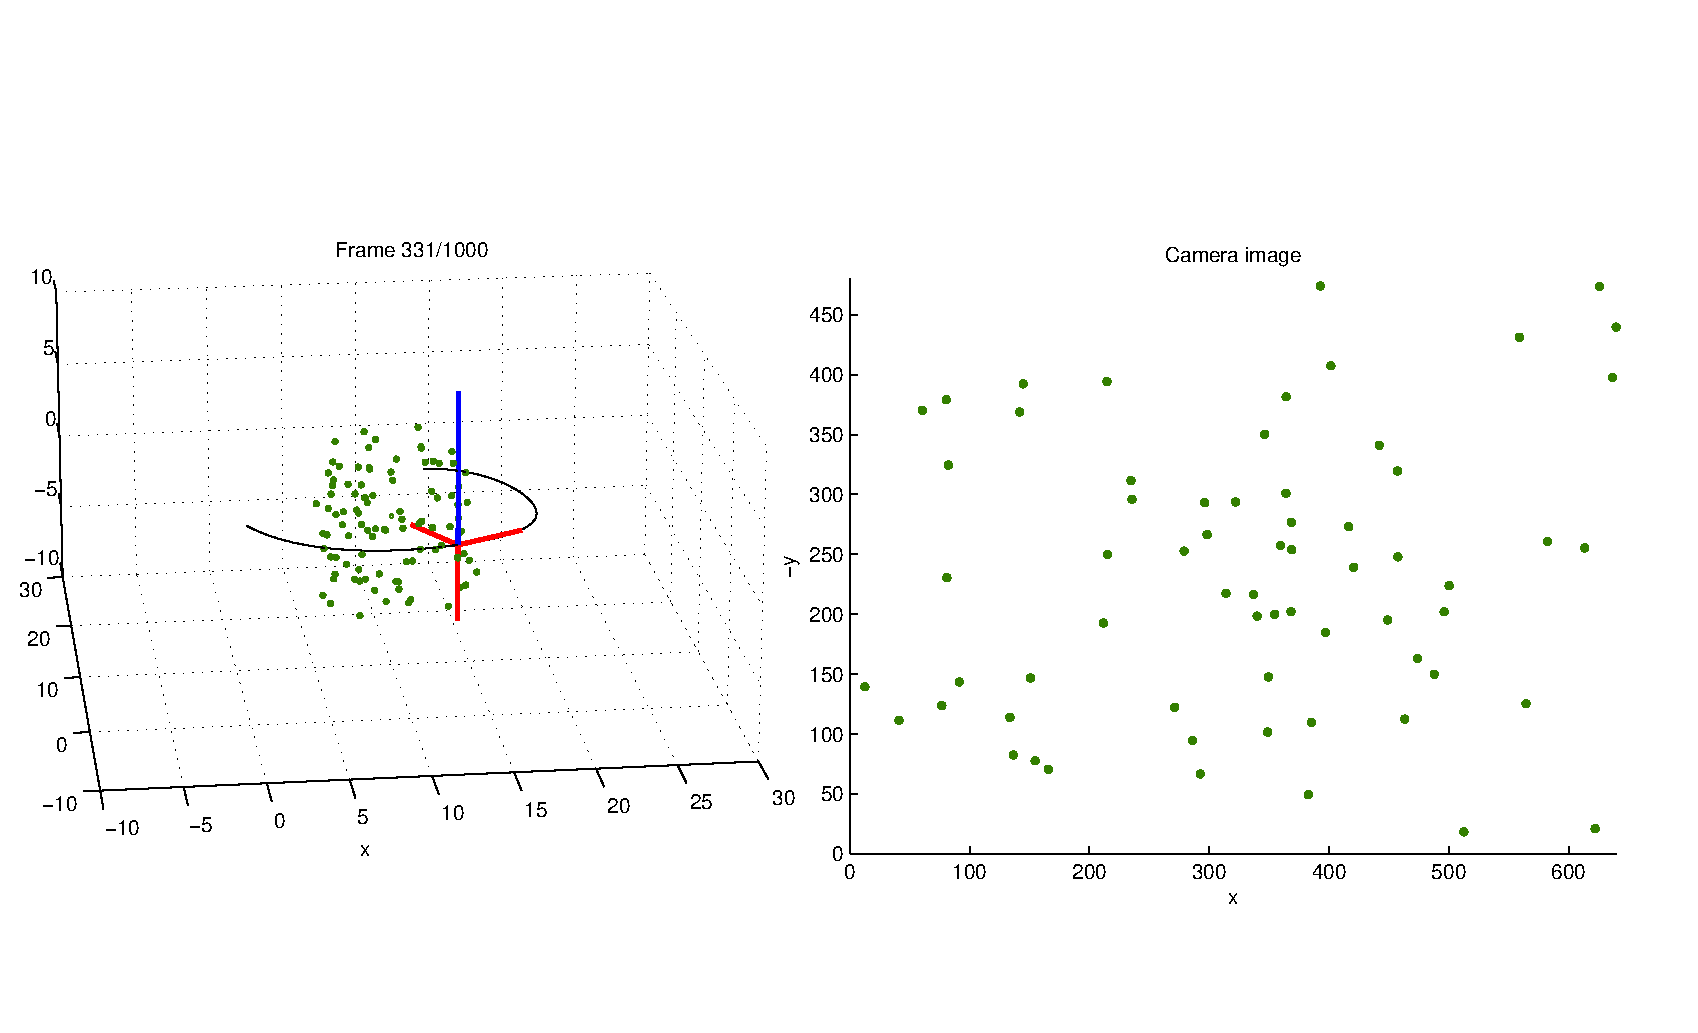
\includegraphics[width=\linewidth]{synth_path.eps}
\caption{Left: Camera path in the world space in black, landmarks in green, IMU-camera setup in blue, camera rotation matrix (look-at, up, and orthogonal vectors) in red. Right: projections of the landmarks in the image plane of the camera.}
\label{synthpath}
\end{figure}